\documentclass{article} % For LaTeX2e
\usepackage{nips13submit_e,times}
\usepackage{hyperref}
\usepackage{url}

% *** GRAPHICS RELATED PACKAGES ***
\usepackage[pdftex]{graphicx}
\usepackage{caption}
\usepackage{subcaption}
% declare the path(s) where your graphic files are
\graphicspath{{./figure/}}
% and their extensions so you won't have to specify these with
% every instance of \includegraphics
\DeclareGraphicsExtensions{.pdf,.jpeg,.png}


\title{LDA Learning Note}


\author{
Jian Wang\thanks{ Use footnote for providing further information about author (webpage, alternative address)---\emph{not} for acknowledging funding agencies.} \\
CAD Center Tongji University\\
Shanghai, China 201804 \\
\texttt{elan2.wang@gmail.com} 
}


\newcommand{\fix}{\marginpar{FIX}}
\newcommand{\new}{\marginpar{NEW}}

\nipsfinalcopy % Uncomment for camera-ready version

\begin{document}


\maketitle

\begin{abstract}
the abstract goes here
\end{abstract}

\section{Introduction}
This document is intended to serve as a note for later reading, also collect some materials for my own paper.
\section{LDA And Its Variations}

\subsection{LDA}
LDA\cite{Blei:2003}, The target of inference is the distribution
\begin{equation}
p\left ( \vec{z}|\vec{w} \right ) = \frac{p\left ( \vec{z}, \vec{w} \right )}{p\left ( \vec{w} \right )}
\end{equation}

\section{Gibbs Sampling Implementation}
Gibbs sampling is a special case of Markov Chain Monte Carlo (MCMC) simulation and often yields simple algorithms for the approximate inference in high dimensional models such as LDA.

Before applying LDA model to process the corpus, we need firstly do some preparation work, such as, remove stop words and infrequent words that appear less than 5 documents. We store all the words appeared in the corpus in the vocabulary.txt file, and the line number corresponds to the index number of the word. So a document is represented as a sequence of numbers.

\section{Gibbs Sampling for Logistic Normal Topic Models}
Previous work on probabilistic topic models has either focused on models with relatively simple conjugate priors that support Gibbs sampling or models with non-conjugate priors that typically require variational inference. Gibbs sampling is more accurate than variational inference and better supports the construction of composite models\cite{mimno2008gibbs}.
\subsection{Logistic Function}
A \textbf{logistic function} or \textbf{logistic curve} is a common \textbf{sigmoid function}. A generalized logistic curve can model the "S-shaped" behavior  (abbreviated S-curve) of growth of some population P. The logistic function is the sigmoid curve with equation:
\begin{equation}
f\left ( x \right ) = \frac{1}{1+e^{-x}} = \frac{e^x}{1+e^x}
\end{equation}
In practice, due to the nature of the \textbf{exponential function} $e^{-x}$, it is often sufficient to compute x over a small range of real numbers such as [-6, +6].  
\subsection{Logit Function}
The \textbf{Logit function} is the inverse of the sigmoidal "logistic" function used in mathematics, especially in statistics. When the function's parameter represents a probability, the logit function returns the log-odds.The \textbf{logit} of a number $p$ between 0 and 1 is given by the formula:
\begin{equation}
logit\left ( p \right ) = log\left ( \frac{p}{1-p} \right ) = log\left ( p \right ) - log\left ( 1-p \right )  
\end{equation}
\subsection{Logistic Distribution}
In probability theory and statistics, the \textbf{logistic distribution} is a continuous probability distribution. Its \textbf{cumulative distribution function} is \textbf{logistic function}. It resembles the normal distribution in shape but has heavier tails. The \textbf{probability density function (pdf)} of the logistic distribution is given by:
\begin{equation}
f\left( x;\mu ,s \right) = \frac{e^{-\frac{x-\mu}{s}}}{s\left(1+e^{-\frac{x-\mu}{s}} \right )^2} = \frac{1}{4s}sech^2\left(\frac{x-\mu}{2s} \right)
\end{equation}
The logistic distribution receives its name from its \textbf{cumulative distribution function(cdf)}, which is an instance of the family of logistic functions.
\begin{equation}
F\left( x;\mu ,s \right) = \frac{1}{1+e^{-\frac{x-\mu}{s}}} = \frac{1}{2}+\frac{1}{2}tanh\left(\frac{x-\mu}{2s} \right)
\end{equation}
In the above two equations, $x$ is the random variable, $\mu$ is the mean, and $s$ is a scale parameter proportional to the standard deviation.
% picture of logistic normal distribution
\begin{figure}[htb]
	\centering
	\begin{subfigure}{0.5\textwidth}
		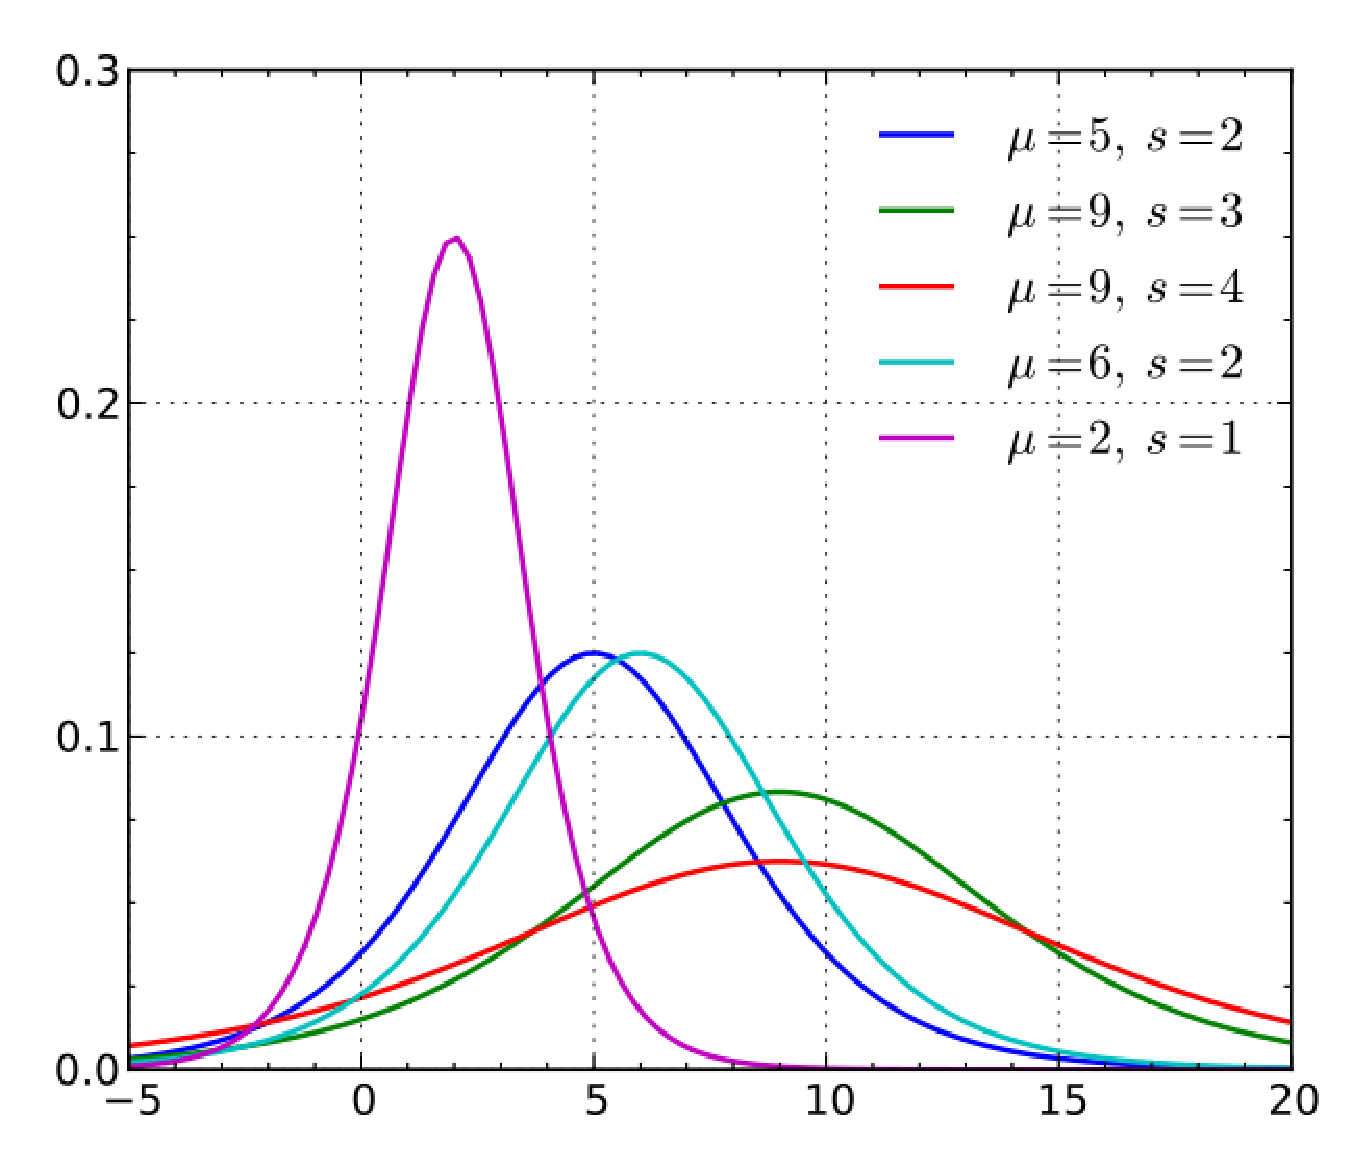
\includegraphics[width=6.5cm]{640px-Logisticpdfunction}
		\caption{probability density function}
	\end{subfigure}%
	\begin{subfigure}{0.5\textwidth}
		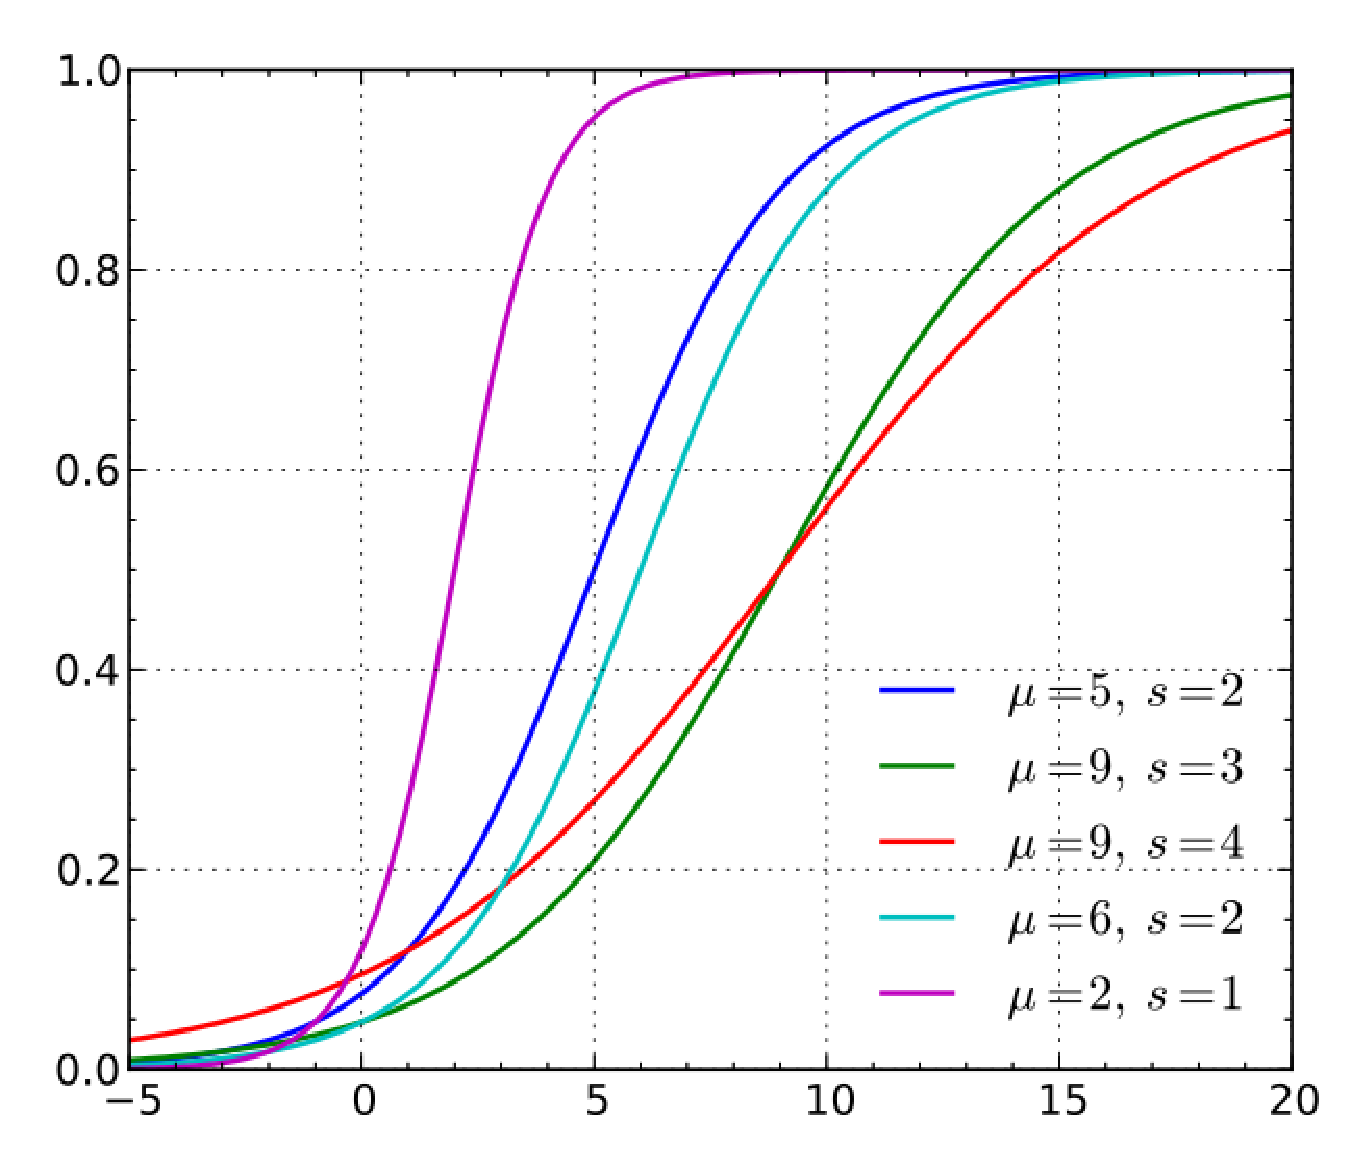
\includegraphics[width=6.5cm]{640px-Logistic_cdf}
		\caption{cumulative distribution function}
	\end{subfigure}
	\caption{pdf and cdf of logistic normal distribution}
\end{figure}

\subsection{Logistic Normal Distribution}
The logistic normal distribution is a distribution on the simplex, obtained by transforming a random variable drawn from a multivariate Gaussian distribution. A point $\theta$ in the $T-1$ simplex (i.e., a $T - 1$ dimensional logistic normal random variable) can be generated as follows:

\begin{enumerate}
\item Generate a $T$-dimensional vector of parameters $\beta \in R^{T}$ from a $T$-dimensional Gaussian distribution with mean $\mu$ and covariance matrix $\Sigma$: $\beta \sim N\left(\beta; \mu, \Sigma \right)$. For identifiability it is common practice to set $\mu$ and $\Sigma$ such that $\beta_{T}$ is guaranteed to be zero.
\item Transform $\beta$ into $\theta$ using the logistic transform: $\theta_{t} = \frac{exp(\beta_{t})}{\sum_{t'=1}^{T}exp(\beta_{t'})} =  \frac{exp(\beta_{t})}{1+\sum_{t'=1}^{T-1}exp(\beta_{t‘})}$
\end{enumerate}

\section{Data Augmentation}
The term \emph{data augmentation} \cite{van2001art} refers to methods for constructing iterative optimization or sampling algorithms via the introduction of unobserved data or latent variables. 

\section{Conclusion}
The conclusion goes here.

% reference
\bibliographystyle{plain}
\bibliography{/Users/wangjian/Dropbox/Papers/library}

\end{document}
